\documentclass{article}

\usepackage{listings}
\usepackage{xcolor}
\usepackage{caption}
\usepackage[a4paper, total={6in, 10in}]{geometry}
\usepackage[utf8x]{inputenc}
\usepackage[framemethod=tikz]{mdframed}

\lstset{
  language=C,               
  numbers=left,             
  stepnumber=1,             
  numbersep=10pt,           
  backgroundcolor=\color{white},
  showspaces=false,             
  showtabs=false,               
  tabsize=2,                    
  captionpos=b,                 
  breaklines=true,              
  breakatwhitespace=true,       
  belowcaptionskip=1\baselineskip,
  breaklines=true,
  xleftmargin=\parindent,
  showstringspaces=false,
  basicstyle=\footnotesize\ttfamily,
  keywordstyle=\bfseries\color{blue!40!black},
  commentstyle=\itshape\color{green!40!black},
  stringstyle=\color{orange},
}

\newcommand\mylstcaption{}

\mdfdefinestyle{mymdstyle}{
hidealllines=true,
middleextra={
  \node[anchor=west] at (O|-P)
    {\lstlistingname~\thelstlisting\  (Cont.):~\mylstcaption};},
secondextra={
  \node[anchor=west] at (O|-P)
    {\lstlistingname~\thelstlisting\  (Cont.):~\mylstcaption};},
splittopskip=2\baselineskip
}

\surroundwithmdframed[style=mymdstyle]{lstlisting}
\newmdenv[style=mymdstyle]{mdlisting}

\begin{document}
\section{Writing a dynamic memory allocator package simulator}
\paragraph{Solution}
The created simulator implements basic functions for a dynamic memory allocator (DMA).
Three main function is based on standard DMA GNU Malloc library for C language:
\begin{itemize}
    \item \begin{verbatim}void *malloc(size_t size);\end{verbatim}
    \item \begin{verbatim}void *realloc(void *p, size_t size);\end{verbatim}
    \item \begin{verbatim}void free(void *p);\end{verbatim}
\end{itemize}
The implementation is based on the explicit free list structure
with boundary tags for coalescing of the adjacent free objects in the heap.
The source code of dynamic package allocator is shown on listing \ref{lst:c1}.
\renewcommand\mylstcaption{.}
\begin{mdlisting}
    \lstinputlisting[caption=\mylstcaption, label=lst:c1]{../mm.c}
\end{mdlisting}
\paragraph{Results}
The program was run against the evaluator which computes memory utilization and package throughout.
The values are displayed as percentage values of the reference GNU Malloc package.
For the most part of the test traces the simulator shows more than 80\% memory utilization (util column)
and good throughout (Kops column). As explicit free list is not the optimal structure 
for DMA it is unable to perform well across all kind of traces. 
Memory utilization lows up to 50\% as well as throughput drops by an order of magnitude for traces with binary allocating patterns. 
And up to 39\% for traces with realloc() calls. But overall it has Perf index equal to 80 out of 100.
The screenshot of the evaluator run is presented on figure \ref{fig:test-run}.
\begin{figure}[h]
    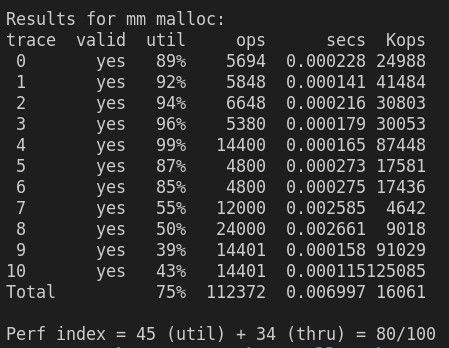
\includegraphics[width=0.6\textwidth]{evaluation.jpg}
    \centering
    \caption{Benchmark results}
    \label{fig:test-run}
\end{figure}
\end{document}